\section{Performance Comparison}

The performance of trading strategies can be compared in many ways.
To reduce complexity, only the three most important metrics are used to compare the result of trading strategies.

Namely, these are \cite{performace}:

\begin{enumerate}
    \item \textbf{Equity Curve}
    \item \textbf{Maximum Drawdown}
    \item \textbf{Win Ratio}
\end{enumerate}

\subsection{Equity Curve}
\label{chap:equity-curve}

The equity curve is one of the simplest and fastest ways to compare trading strategies.
It is a visual or graphical representation of the account equity over the backtested period.
A gradually upward sloping equity curve is more preferred than a curve which is very volatile \cite{performace}.

\autoref{fig:equity-curve} shows two different equity curves.
Even if the more volatile one (orange) is better in the beginning, there are many resets, which causes are worse result compared to the more stable one (blue).

\begin{figure}[H]
    \centering
    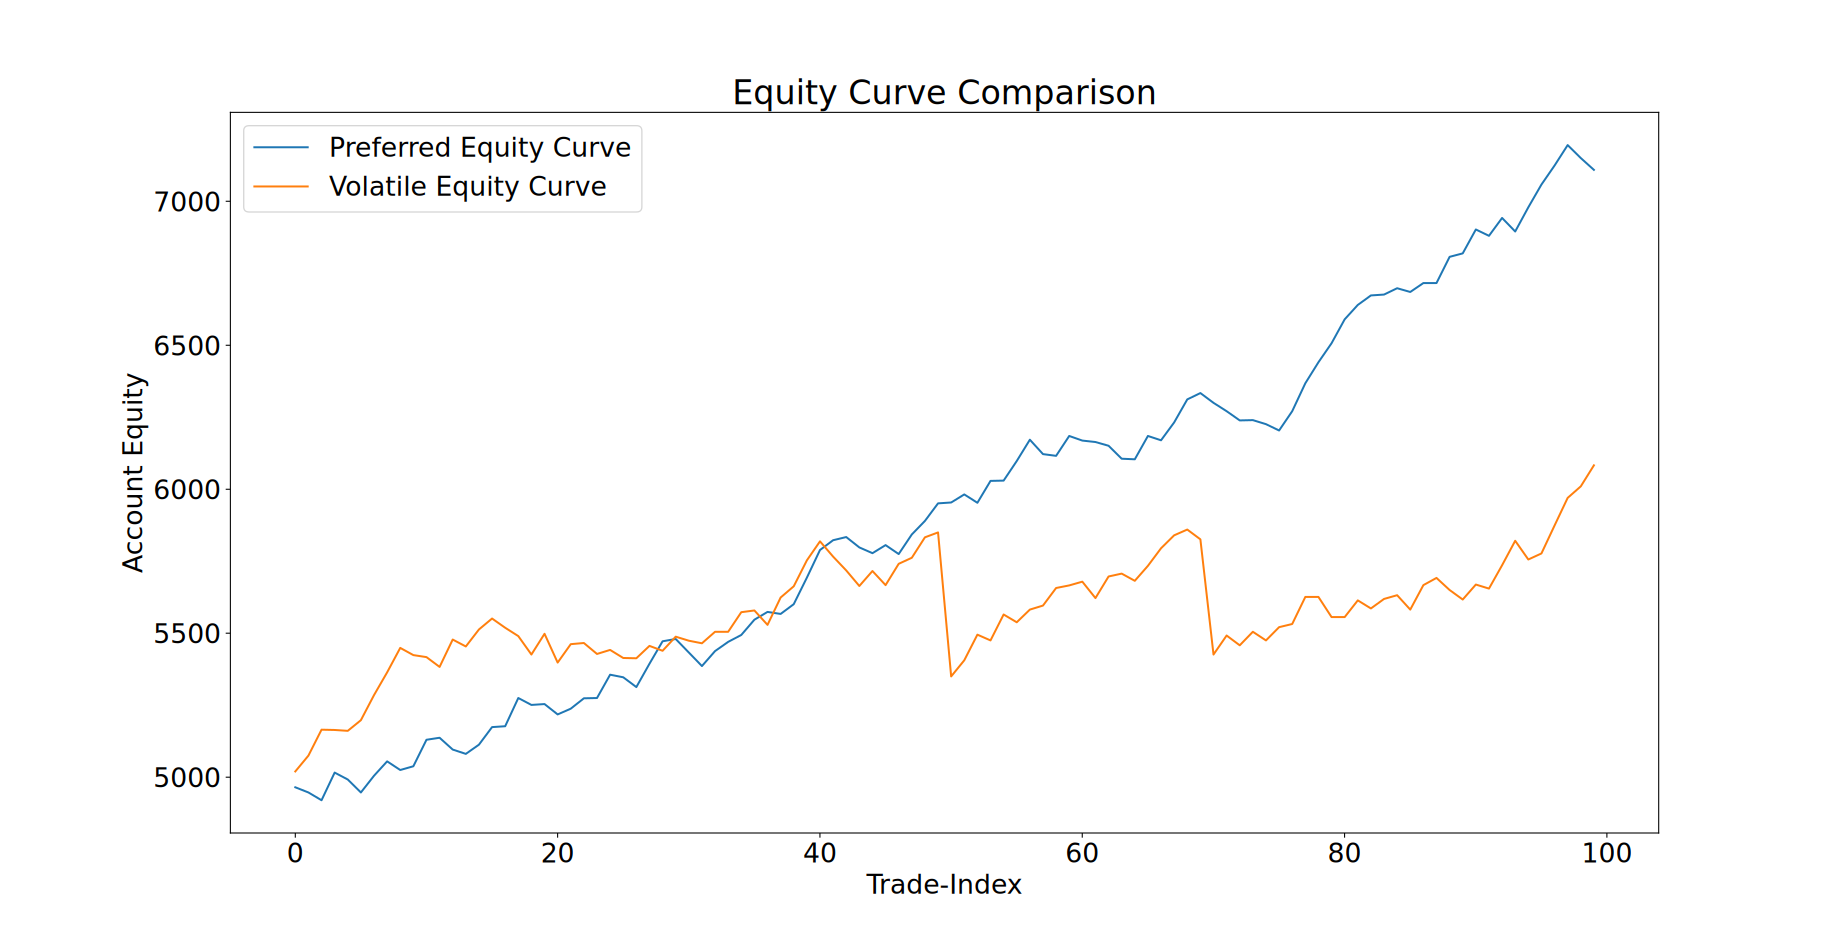
\includegraphics[width=\textwidth]{images/trading-strategies/equity-curve}
    \caption{Equity Curve Comparison}
    \label{fig:equity-curve}
\end{figure}

\subsection{Maximum Drawdown}

The maximum drawdown (MDD) measures the largest percentage loss of an investment from its highest point (peak) to its lowest point (trough) within a specific period.
It shows the maximum amount of a trading strategy lost before the investment recovers.
The MDD is an important risk measure because it highlights the potential losses in times of crisis.
A high drawdown indicates high volatility or poor risk management \cite{mdd}.

For each time-point in the equity curve, the drawdown (DD) at time $t$ can be calculated by \cite{dd}:

\[
    DD_t = \frac{Equity_t - PeakValue_{Before\~t}}{PeakValue_{Before\~t}}
\]

\noindent
The maximum drawdown is then the minimum of all drawdowns.

\autoref{fig:max-drawdown} shows the drawdown curves for both equity curves from \autoref{chap:equity-curve}.
It is noticeable that the maximum drawdown for the more volatile equity curve is much bigger, which also indicates a not optimal trading strategy.

\begin{figure}[H]
    \centering
    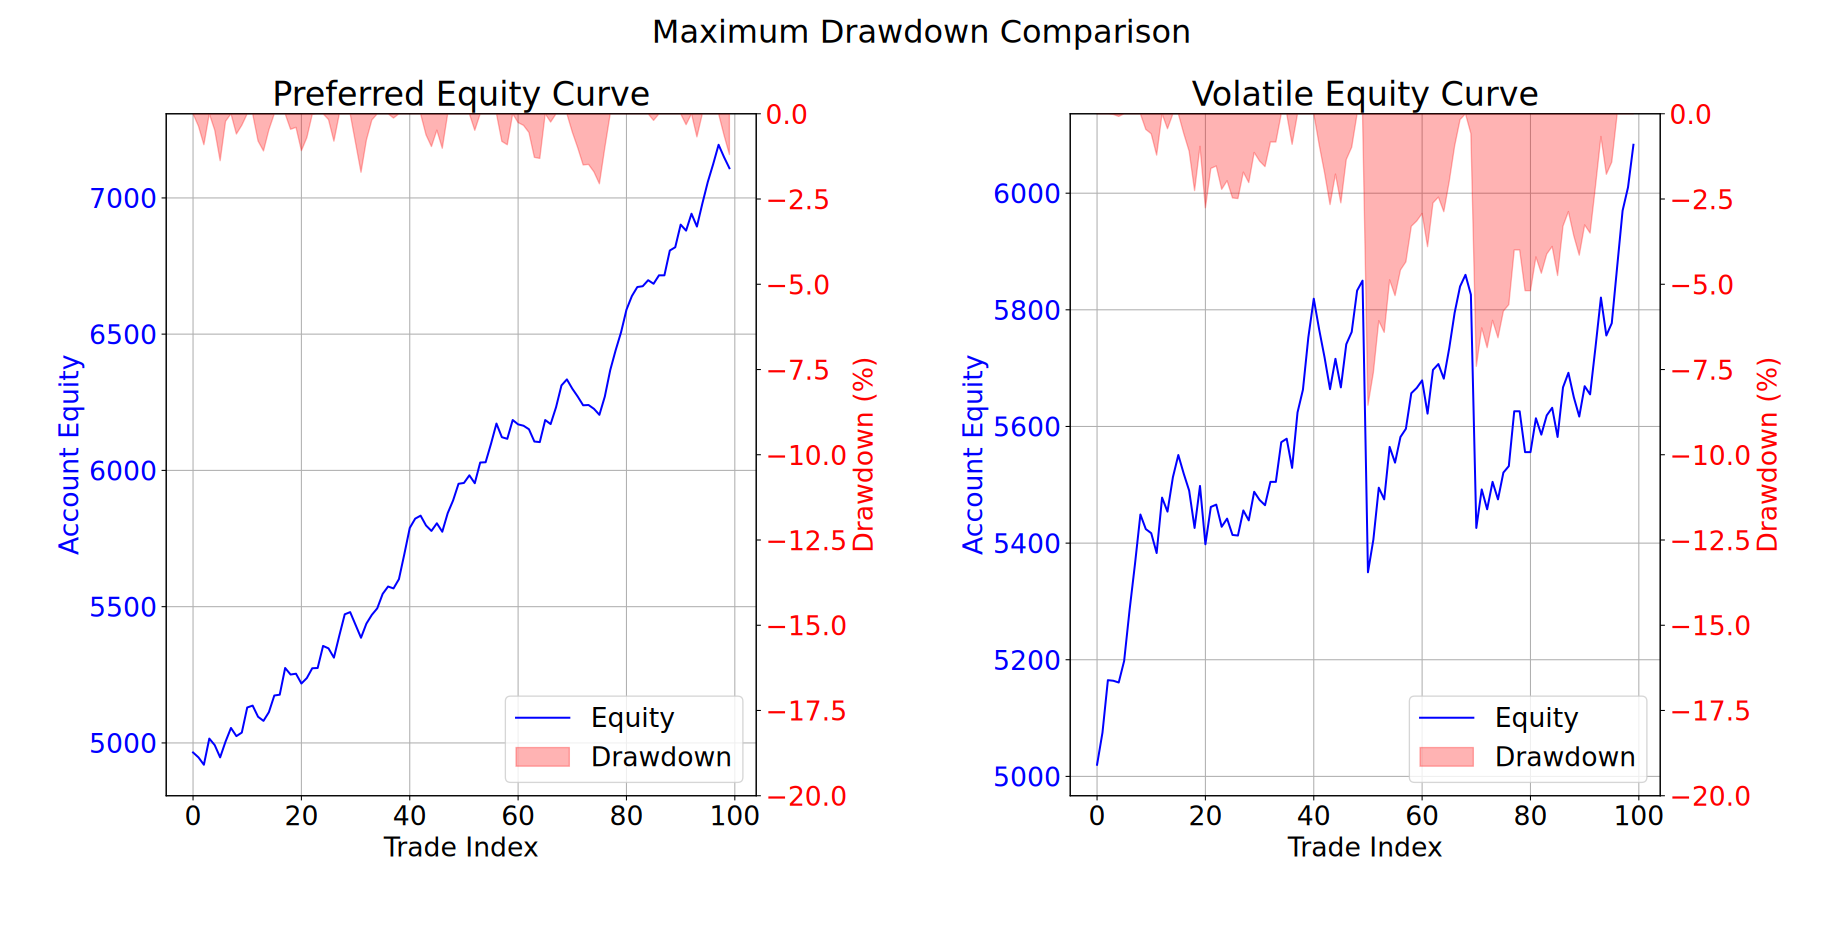
\includegraphics[width=\textwidth]{images/trading-strategies/max-drawdown}
    \caption{Drawdown Comparison}
    \label{fig:max-drawdown}
\end{figure}

\subsection{Win Rate}
\label{chap:win-rate}

Another interesting metric for trading strategy comparison is the win rate (or win ratio).
It is the percentage of profitable trades in relation to the total number of trades and is calculated as follows:

\[
    WinRate = \frac{Number Of Winning Trades}{Total Number Of Trades} * 100
\]

\noindent
For example, if for a total of 20 trades, 16 have been profitable, the win rate is $\frac{16}{20} * 100 = 80\%$.

The greatest limitation of the win rate is that a high win rate does not always indicate a profitable trading strategy \cite{win-rate}.
For example, if the win rate is 80\% with an average gain of 20\$ per profitable trade and an average loss of 90\$ per unprofitable trade, the weighted average is $\frac{80 * 20 - (100 - 80) * 90}{100} = -2$\$.
Assuming a different strategy with 40\% win rate, but with an average gain of 70\$ per profitable trade and an average loss of 15\$ per unprofitable trade, its weighted average is $\frac{40 * 70 - (100 - 40) * 15}{100} = 19$\$.
The second strategy has a much lower win rate, but its long-term outcome is much higher, compared to the first one.